\documentclass[a4paper,11pt]{article}
\usepackage[margin=19mm,top=19mm,bottom=20mm,headheight=14pt,headsep=5mm]{geometry}
\usepackage{fontspec}
% Calibri is supplied by the user's licensed local Windows installation.
% Font binaries are not distributed in the source archive.
\providecommand{\GuideFontPath}{.build/fonts/}
\defaultfontfeatures{Ligatures=TeX}
\setmainfont{calibri.ttf}[Path=\GuideFontPath,BoldFont=calibrib.ttf,ItalicFont=calibrii.ttf,BoldItalicFont=calibriz.ttf]
\setsansfont{calibri.ttf}[Path=\GuideFontPath,BoldFont=calibrib.ttf,ItalicFont=calibrii.ttf,BoldItalicFont=calibriz.ttf]
\setmonofont{calibri.ttf}[Path=\GuideFontPath,BoldFont=calibrib.ttf,ItalicFont=calibrii.ttf,BoldItalicFont=calibriz.ttf]

\usepackage{microtype,graphicx,xcolor,tikz,pgfplots,fancyhdr,enumitem,booktabs,tabularx,hyperref,xurl,caption,titlesec}
\usetikzlibrary{positioning,arrows.meta,calc,fit,backgrounds}
\usepgfplotslibrary{groupplots}
\pgfplotsset{compat=1.18}
\definecolor{ink}{HTML}{173042}
\definecolor{teal}{HTML}{007E87}
\definecolor{pale}{HTML}{EEF5F6}
\definecolor{muted}{HTML}{596A77}
\definecolor{orange}{HTML}{B96812}
\definecolor{red}{HTML}{AA3B4A}
\hypersetup{colorlinks=true,linkcolor=black,urlcolor=black,citecolor=black,pdftitle={A Factory Alarm, Explained: An Engineer's Guide to Meta-Harness},pdfauthor={Local Meta-Harness Project}}
\setlength{\parindent}{0pt}
\setlength{\parskip}{6pt}
\setlength{\emergencystretch}{3em}
\raggedbottom
\setlist{leftmargin=*,topsep=4pt,itemsep=3pt,parsep=0pt}
\titleformat{\section}{\sffamily\bfseries\LARGE\color{black}}{}{0pt}{}
\titlespacing*{\section}{0pt}{0pt}{7pt}
\titleformat{\subsection}{\sffamily\bfseries\large\color{black}}{}{0pt}{}
\titlespacing*{\subsection}{0pt}{9pt}{4pt}
\pagestyle{fancy}
\fancyhf{}
\renewcommand{\headrulewidth}{0pt}
\fancyhead[L]{}
\fancyhead[R]{}
\fancyfoot[L]{}
\fancyfoot[R]{\color{black}\sffamily\small\thepage}
\captionsetup{font=small,labelfont={sf,bf},skip=5pt,hypcap=false,justification=raggedright,singlelinecheck=false}
\urlstyle{same}
\newcommand{\page}[2]{\clearpage\thispagestyle{fancy}\noindent{\sffamily\small\bfseries\color{black}#1}\par\vspace{3mm}\section*{#2}}
\newcommand{\takeaway}[1]{\par\smallskip\begingroup\setlength{\fboxsep}{8pt}\colorbox{pale}{\parbox{\dimexpr\linewidth-16pt\relax}{\raggedright\sffamily\small\textbf{Remember.} #1\par}}\endgroup\par\smallskip}
\newcommand{\evidence}[1]{\par\smallskip{\raggedright\footnotesize\color{black}\textbf{Basis:} #1\par}}
\newcommand{\diagram}[2]{\begin{center}\input{guide/figures/#1.tex}\captionof{figure}{#2}\end{center}}
\tikzset{box/.style={draw=teal!65,rounded corners=2pt,fill=pale,align=center,font=\sffamily\small,inner sep=6pt,minimum height=10mm,text=black,execute at begin node={\hyphenpenalty=10000\exhyphenpenalty=10000}},dark/.style={box,fill=gray!12,text=black,draw=ink},arr/.style={-{Stealth[length=2mm]},draw=muted,thick},lab/.style={font=\sffamily\scriptsize,fill=white,inner sep=2pt,align=center,text=black}}
\begin{document}
{\sffamily\small\bfseries\color{black}A SHORT MANUAL FOR GENERAL ENGINEERS | 10 OCTOBER 2026}\par\vspace{4mm}
{\sffamily\bfseries\color{black}\fontsize{27}{31}\selectfont A factory alarm, explained\par}
\vspace{3mm}
{\sffamily\large From the animated line to an operator's next decision\par}
\vspace{5mm}
Imagine arriving at a line you have never worked on. Material enters at the top, screws turn, and parcels move along the conveyor. Then a component flashes, a technician walks across the scene, and an AI investigation appears. What actually happened?

This guide follows that story without assuming extrusion or AI experience: meet the machine, follow an alarm, and learn what inspection, repair and restart mean. Then meet the agent backstage: how it gets advice, uses evidence and earns permission to act.

\begin{center}
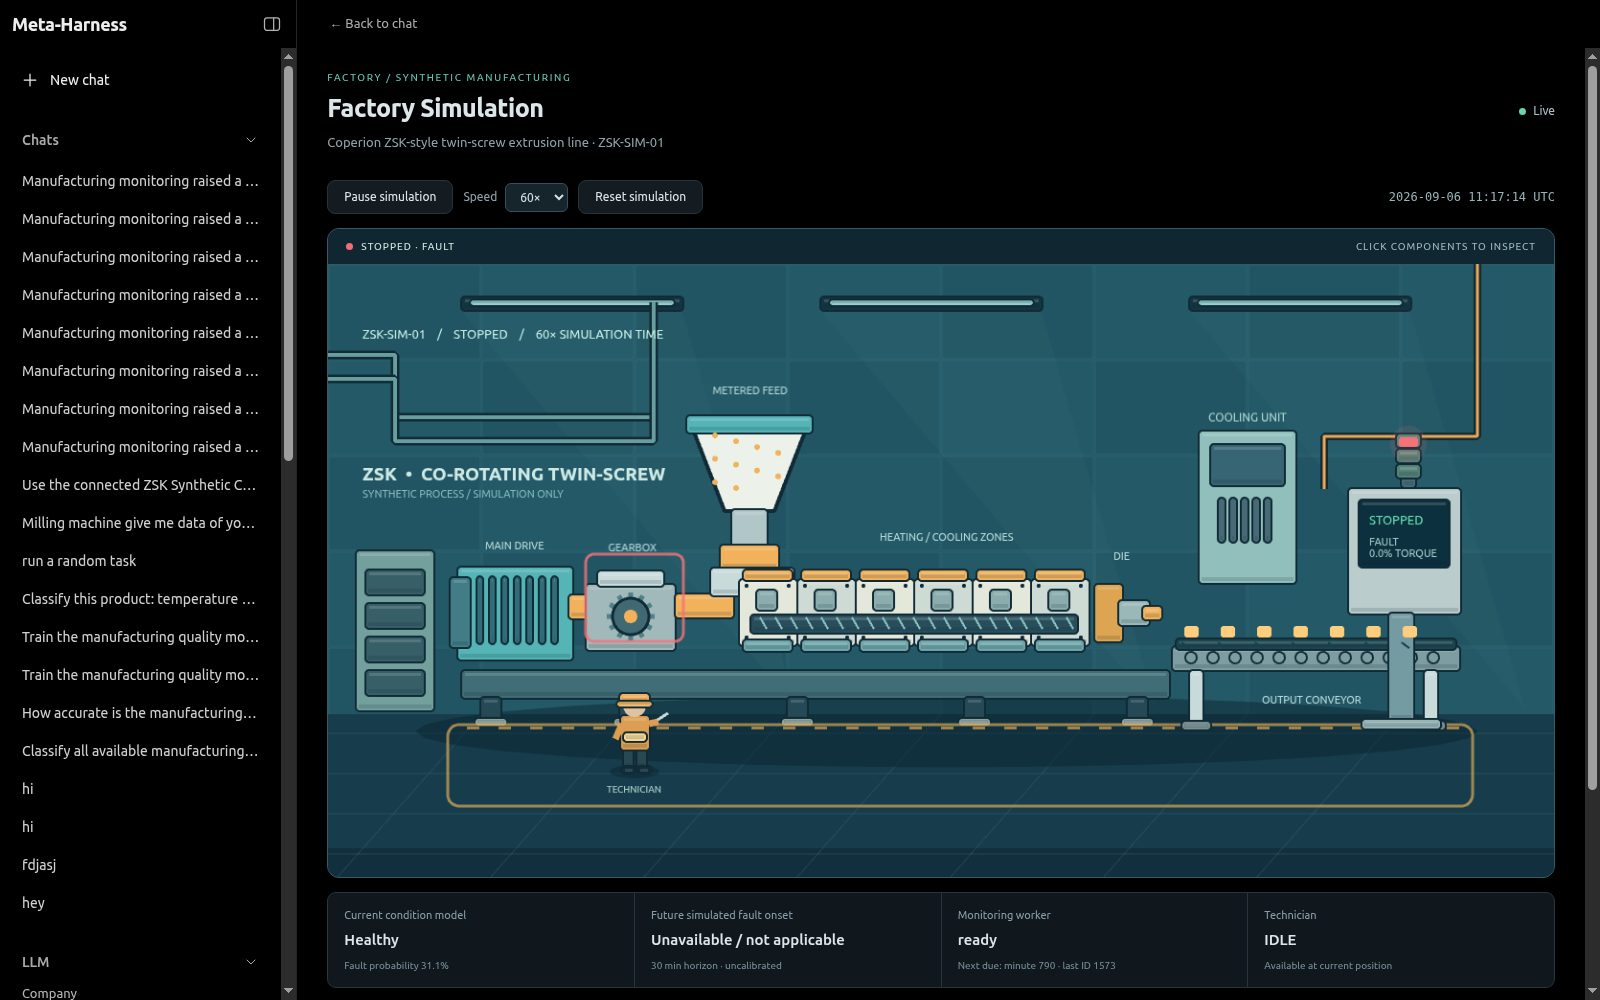
\includegraphics[width=.95\linewidth,trim=327bp 122bp 46bp 228bp,clip]{guide/figures/game-scene.png}
\captionof{figure}{The actual game in a saved browser verification capture: STOPPED / FAULT. The displayed machine is synthetic; no physical line is connected.}
\end{center}

\takeaway{The game displays a synthetic machine. The backend owns its condition, sensors and actions; the AI investigates its records. No physical manufacturing line is connected.}

\subsection*{Follow the story}
\begin{tabularx}{\linewidth}{@{}rXrX@{}}\toprule
2 & Meet the line & 10 & Connect the agent to the LLM\\
3 & Read the signals & 11 & Follow the agent's loop\\
4 & Understand the two models & 12 & Tools and security\\
5 & Watch an investigation & 13 & Consult documents with RAG\\
6 & Understand the animation & 14 & Memory and context\\
7 & Follow a recorded alarm & 15 & Validate and recover\\
8 & Inspect, repair, restart & 16 & Find help and sources\\
9 & Try different problems & & \\\bottomrule
\end{tabularx}

The ZSK-style extruder and its fault effects are illustrative, not a manufacturer maintenance procedure.

\page{1 / MEET THE MACHINE}{A mixer with three connected jobs}
Stand in front of the game and read it from left to right. The motor is the source of rotation. The gearbox passes that rotation to two screws inside the barrel. Above them, the hopper holds material and the feeder controls how much enters. The screws carry and mix the material; the barrel's heating and cooling regulate temperature. Material then leaves through the die, the outlet restriction, toward the displayed conveyor.

Three things travel through this arrangement: \textbf{material}, \textbf{mechanical power}, and \textbf{heat}. They interact, but they are different flows. The diagram separates them so an arrow from the motor cannot be mistaken for a material pipe.
\diagram{line}{Functional map of the game's line. Solid teal arrows carry material; dashed dark arrows carry mechanical power; orange arrows show thermal influence. Positions are schematic, not a construction drawing.}

\subsection*{What each part tells the engineer}
\begin{tabularx}{\linewidth}{@{}p{.19\linewidth}p{.24\linewidth}X@{}}\toprule
Look at & Read & Ask\\\midrule
Motor & Current (A), power (kW) & Is the drive working harder?\\
Gearbox & Vibration (mm/s RMS), oil temperature (°C) & Has shaking or oil heating changed?\\
Screws / barrel & Speed (rpm), torque (\%), barrel temperature (°C) & Is resistance or thermal control changing?\\
Feeder & Feed rate (kg/h) & Is material arriving steadily?\\
Outlet / die & Pressure (bar), melt temperature (°C) & Is downstream resistance or melt condition changing?\\\bottomrule
\end{tabularx}

If the outlet becomes more restrictive, pressure and screw torque can rise together. That does not automatically mean the gearbox is damaged. Follow the interacting readings before choosing an inspection.

\takeaway{Clicking a drawn component opens its details. It does not diagnose or repair it. The model receives ten numerical signals, not a picture of the machine.}
\evidence{Game component map: \path{factory-service/factory/domain.py}. Signal definitions and scenario effects: \path{zsk-service/zsk/synthetic.py}. The software stores one barrel-temperature signal, not separate readings for every drawn heating zone.}

\page{2 / READ THE HISTORY}{A rising line needs context}
Open \textbf{Machine Monitoring}. Each stored point is a reading, not a frame of animation. The live simulator samples every five simulated minutes. Compare signals over time and under comparable loading; one high value alone does not identify a failed component.

The chart below uses the original supplied history, \textbf{not the live game's current episode}. Recipe A/B/C describes the operating recipe. Recipe changes can shift the baseline, so their boundaries are marked across all panels.
\diagram{history}{All 1,000 original synthetic readings, 1--4 September 2026. Torque, gearbox vibration and oil temperature share time, with separate units and scales. The bottom panel contains supplied health labels, not ML predictions. Labels remain in the source CSV; the initial training labels were purged from the runtime database.}

Lines connect recorded sensor points; they do not measure between samples. The label step trace holds each supplied tag until the next reading. No smoothing, resampling or manufacturer alarm threshold has been added. The two vertical markers indicate recipe changes, not inferred failures.

\takeaway{Use a trend to decide what to investigate. Keep the timestamp, recipe, units and production state with the value. A reading from a stopped drive is not a healthy running baseline.}
\evidence{Exact source: \path{zsk-service/data/zsk_labeled_1000.csv}. First/last timestamps: 1 Sep 00:00 / 4 Sep 11:15 UTC; 83 h 15 min total. All plotted values and five-minute intervals are checked by \path{guide/build_data.py}.}

\page{3 / UNDERSTAND THE MODELS}{Two questions, two different answers}
Back in the game, look below the scene. \textbf{Current condition} asks whether the observed pattern resembles synthetic Healthy or Faulty examples. \textbf{Future simulated fault onset} asks whether a still-healthy simulated machine may develop a fault within the registered horizon, usually 30 minutes. It does not estimate remaining machine life.

Both machine-learning (ML) models use ten signals, recipe indicators and recent statistics. A full window contains the current reading and two earlier readings: at five-minute spacing, the first and last are ten minutes apart. Neither receives simulator severity or a hidden fault name as an input.

\subsection*{Read the errors as well as the score}
\diagram{matrices}{Recorded chronological evaluations on two different synthetic datasets. Rows are actual classes; columns are model decisions; each panel contains 200 cases. The meanings of 0/1 differ between the models, so words replace numeric class codes.}

For current condition, the candidate missed \textbf{2 of 46 faulty readings} and raised \textbf{4 false alarms among 154 healthy readings}. It scored 97\% overall, but that does not mean 97\% accuracy on a real extruder. The deployed current classifier was subsequently fitted on all 1,000 labeled source rows; the plot evaluates the earlier candidate.

For future onset, the separate model missed \textbf{9 of 30 onsets} and raised \textbf{5 false alarms among 170 no-onset cases}. The evaluated forecast candidate itself was deployed without fitting its holdout. Its 30-minute prediction is unavailable when the current classification is Faulty, the line is not running, or three continuous readings are missing.

\takeaway{The game's FAULT/WARNING light comes from simulator fault severity. Healthy/Faulty below the scene comes from ML. They can disagree. A probability is a synthetic model output, not a confirmed diagnosis or calibrated industrial risk.}
\evidence{Current matrix: \path{evidence/zsk-final-state.json}. Future-onset matrix: \path{docs/verification/factory/forecast-metrics.json}. These saved results were not reevaluated for this rewrite.}

\page{4 / FOLLOW THE ALARM}{The machine raises a question}
Now inject gradual gearbox vibration in \textbf{Simulation Settings}. As simulated time advances, the programmed effect changes vibration and oil temperature. The worker stores readings and periodically sends them to the ML service. A Faulty classification, or a future-onset score at or above the configured threshold, can create an alarm. Fault injection itself is not an ML alarm.
\diagram{investigation}{The actual automatic path. The simulator owns measurements and alarm delivery; the existing core task engine owns AI execution. The browser watches this path rather than running it.}

The backend assigns the alarm a \textbf{component hypothesis} using fixed signal checks. The AI then retrieves the records and saved predictions, searches documentation for the configured demonstration asset, and chooses permitted tools. RAG means retrieving relevant passages from stored documents; it is the agent's reference shelf, not a separate diagnosis engine.

The task template requires a completed inspection of the alarm's assigned component. The inspection tool starts a backend action and moves the technician automatically. The agent must check the returned action's status, matching episode, component and alarm, before claiming that inspection is complete. If both its grant and backend policy allow a simulated stop, it can stop the line and verify STOPPED.

\subsection*{What completion proves}
For the stop demonstration, fixed checks require sensor records, saved ML output, nonempty scoped documentation, a completed matching inspection, STOPPED production and the correct episode. These checks establish recorded software facts. They do not judge whether the cited passage proves a mechanical cause.

\takeaway{The agent's report should separate observations, model results, sources, possible causes, completed actions and uncertainty. A plausible explanation is still a hypothesis.}
\evidence{Monitoring and alarm path: \path{factory-service/factory/worker.py}. Required task evidence and grants: \path{core/config/task-integrations.json}. The configured RAG asset is an explicit demo mapping, not verified physical machine identity.}

\page{5 / WATCH THE GAME}{What the moving technician really means}
Click the gearbox in \textbf{Factory Simulation}. Its inspector panel opens below the scene. Pressing \textbf{Send technician to inspect} submits an actual simulation action. The backend records the job and destination; the character walks to the component; the backend eventually records a completed observation. An accepted request is only the start of this sequence.

\begin{center}
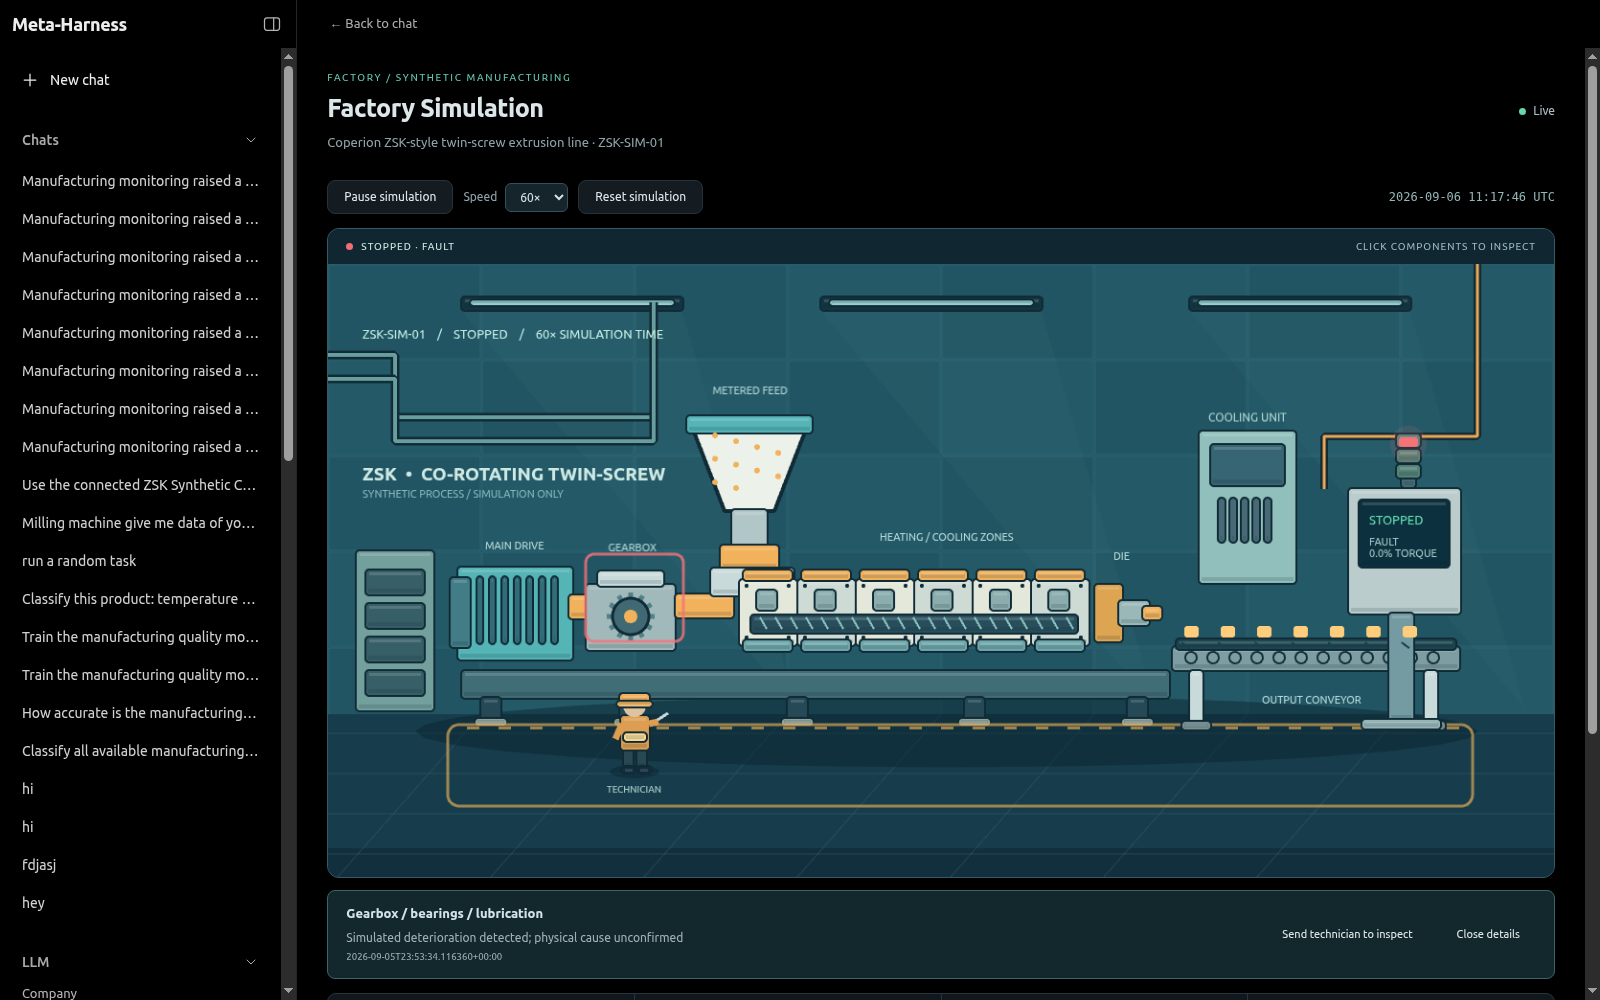
\includegraphics[width=\linewidth,trim=327bp 20bp 46bp 540bp,clip]{guide/figures/game-inspector.png}
\captionof{figure}{Saved game capture: technician at the gearbox, inspector open below the scene. The finding is synthetic deterioration, not a physical diagnosis. This is earlier verification evidence, not a new run.}
\end{center}

\subsection*{Read the scene without overreading it}
\begin{tabularx}{\linewidth}{@{}p{.30\linewidth}X@{}}\toprule
What you see & What the software actually does\\\midrule
Gears, screws and parcels move & Phaser draws generic motion from production mode and simulated time, not a calibrated physical model.\\
The technician walks or works & The backend owns position and job status. The browser smooths movement between snapshots.\\
A component flashes & The scene uses the alarm component, with a gearbox fallback before an alarm exists. Flashing alone is not diagnosis evidence.\\
An inspection finding appears & The backend checks injected scenarios for that component and returns a synthetic observation, not a mechanical test.\\\bottomrule
\end{tabularx}

\textbf{Pause simulation} freezes the simulated clock and pending actions. \textbf{Stop simulated line} stops production, but the clock can keep running so diagnostics finish. The backend runs even when the browser is closed. At 60×, ten simulated minutes take ten wall-clock seconds; the AI's response time is still real elapsed time.

\takeaway{The AI reads structured tool results, not the game image. The animation makes those results visible. Different faults mostly share the same machinery animation; the sensor records and inspection results distinguish them.}
\evidence{Rendering: \path{ui/src/components/factory/factory-scene.ts}. Clock, technician movement and inspection results: \path{factory-service/factory/domain.py}.}

\page{6 / A RECORDED EPISODE}{From shaking to an operator report}
Here the story becomes a saved execution record. In a gradual gearbox scenario, six retrieved readings showed rising vibration, oil temperature and motor current while the line was running. The plots use their exact five-minute timestamps and values. This is a previously completed demonstration, not a new run made for this manual.
\diagram{episode}{Six saved readings from 5 September 2026, 22:19--22:44 UTC (simulated time). Dots are measurements; lines only connect them. The vertical marker is alarm-time reading 1420 at 22:29 UTC, not an invented sensor limit.}

At the alarm, vibration was \textbf{3.001 mm/s RMS}, oil temperature \textbf{49.423°C}, and current \textbf{79.262 A}. The current model returned Faulty with probability \textbf{0.60442}; future-onset forecasting was not applicable. Retrieved publication passages described vibration/oil monitoring, providing context rather than confirming a bearing failure.

The agent inspected the gearbox, checked completion, executed the permitted simulated stop and acknowledged the alarm. Its fixed checks passed. The final state was \textbf{STOPPED / FAULT}: the investigation finished, but the injected fault remained. Later zero speed, current and vibration reflected stopped production, not repair.

\takeaway{A useful report tells the operator what changed, what was checked and what still needs investigation. This episode supports an inspection recommendation; it does not prove a physical root cause.}
\evidence{Task \texttt{306f5c12-5c55-486c-9d5b-5670fb5cf506}; six readings 1418--1423 in the saved \texttt{get\_machine\_measurements} result. Sources: \path{docs/verification/factory/end-to-end.json} and \path{operator-report.md} in that same verification directory.}

\page{7 / FINISH THE STORY}{Inspection is not repair}
The technician has returned to IDLE and the task says COMPLETED. It is tempting to restart. But read both status words: \textbf{STOPPED} describes production; \textbf{FAULT} describes the unresolved simulated deterioration. Completing an investigation changes neither into a repaired machine.
\diagram{repair}{Current operator path for a gearbox scenario. Acknowledging the alarm records receipt; it is not a repair step. Repair and restart are explicit simulation actions, separate from the completed AI investigation.}

\subsection*{What the operator can do in the current game}
After stopping production and obtaining a completed component inspection, the operator can use \textbf{Simulation Settings → Simulate gearbox repair}. The backend removes the active gearbox scenarios, runs the maintenance job, and leaves production stopped. Residual vibration/oil effects decay gradually while simulated time advances. \textbf{Restart simulated line} is a separate confirmed action and rejects severe faults or unfinished jobs.

The current button repairs only the gearbox. Other components have backend maintenance support but no corresponding settings-page repair button. The operator interface is incomplete for those faults.

By default, automatic stop, restart and maintenance are disabled. The explicitly configured stop demonstration grants stop and inspection, not automatic repair or restart. An AI request cannot create those permissions.

\subsection*{Three outcomes to keep separate}
\begin{tabularx}{\linewidth}{@{}p{.24\linewidth}X@{}}\toprule
Investigation complete & Required evidence and actions were recorded.\\
Repair complete & The backend removed the selected programmed fault.\\
Alarm resolved & The worker received qualifying fresh running healthy model evidence with below-threshold future risk after a completed/cancelled investigation.\\\bottomrule
\end{tabularx}

\takeaway{The demonstration can remove a programmed fault. It cannot verify or repair physical equipment. Resetting clears the experiment into a new episode; it is not evidence that a maintenance diagnosis was correct.}
\evidence{Action preconditions and repair transitions: \path{factory-service/factory/domain.py}. Current buttons: \path{ui/src/components/factory/factory-workspace.tsx}. Alarm recovery rule: \path{factory-service/factory/worker.py}.}

\page{8 / TRY ANOTHER PROBLEM}{Why the story can keep returning to the gearbox}
You select unstable feeding, but the report still talks about a gearbox. First check whether you changed the experiment or only the dropdown. Selecting a name does nothing until you click \textbf{Inject simulated fault}. Injection adds a scenario; it does not replace an earlier one.

Automatic scenarios are on by default. The first automatic fault is gearbox vibration after about 60 simulated minutes of a fresh running episode. If that incident remains unresolved, the worker suppresses new alarms for the episode and retains its original component hypothesis. You may therefore be reading the same completed report after adding another fault.

\subsection*{The component selector is deliberately simple}
It first checks vibration above 1.9 mm/s or gearbox oil above 54°C, then pressure above 120 bar, current above 110 A, and barrel-temperature deviation above 15°C. Otherwise it chooses the barrel. These are fixed synthetic routing checks, not manufacturer limits. There is no feeder branch.

\begin{tabularx}{\linewidth}{@{}Xll@{}}\toprule
Single injected scenario & Scenario component & Rule chose\\\midrule
Gearbox vibration & Gearbox & Gearbox\\
Bearing deterioration & Gearbox & Gearbox\\
Oil overheating & Gearbox & Gearbox\\
Excessive screw torque & Barrel & Motor\\
Barrel instability & Cooling & Barrel\\
High melt pressure & Die & Die\\
Unstable feeding & Feeder & Barrel\\
Excessive motor current & Motor & Motor\\\bottomrule
\end{tabularx}
\par{\raggedright\small This isolated source check uses one gradual fault at minute 60, started at minute 0 with a 60-minute duration and seed 13. It checks the fixed routing rule, not ML detection or an end-to-end diagnosis. Earlier readings and combined faults can select differently.\par}

\subsection*{Run a clean comparison}
\begin{enumerate}
\item Wait for pending actions to finish, then confirm \textbf{Reset simulation}. It preserves history and starts a new, paused episode.
\item Turn \textbf{Automatic scenarios} off. Select one fault and press \textbf{Inject simulated fault} while still paused.
\item Set the speed and \textbf{Resume simulation}. Allow time for sampling, monitoring and AI investigation.
\item Open the new episode's alarm and task. Compare its timestamp, component, readings and inspection result; repeat with a reset for the next fault.
\end{enumerate}
\takeaway{The task must inspect the component attached to its alarm. The current routing and incident-retention rules limit scenario-specific advice; this manual does not claim those limitations have been fixed.}

\page{9 / LOOK BACKSTAGE}{Who thinks, who acts, who keeps the record?}
The gearbox flashes in the game. Behind it, several specialists have different jobs. The factory service owns the simulated machine and technician. The ML service evaluates readings. RAG finds document passages. Core coordinates the investigation and keeps its record.
\diagram{architecture}{Current ownership and communication. All services inside the dashed local boundary run locally; OpenAI inference is remote. The arrows show requests and returned results, not sensor or material flow. PostgreSQL stores are separate except that factory and ZSK share the dedicated manufacturing database.}

\subsection*{Connecting the agent to the LLM}
Think of the LLM as an analyst whom the coordinator consults. Core connects to OpenAI using the saved model and settings. It sends the task, relevant context and descriptions of permitted tools. The model returns an explanation or a proposed next step; core handles actual execution.

The connection key stays in backend secret configuration. The browser sees a masked key, and external tools do not need that key. Connection or unsupported-setting failures are shown; the application does not silently substitute another model.

\subsection*{Two different kinds of intelligence}
The ML models score sensor patterns; the LLM chooses investigation steps and explains evidence. The LLM does not run the machine's clock or control the animation. There is one existing agent/model connection, reused by chat and persistent tasks.

\takeaway{The services and records are local, but LLM inference is remote. Relevant observations and retrieved passages supplied as context can leave the local machine.}
\evidence{Current service boundaries and saved-model connection: Factory architecture, Local architecture and API specification; source paths are on page 16.}

\page{10 / FOLLOW THE AGENT}{One step, one result, then another decision}
The alarm opens a persistent investigation. Imagine an engineer working through a checklist: read the alarm, ask for measurements, compare the model result, consult a manual, then decide whether an inspection is needed. The agent follows the same rhythm.

\diagram{agent-loop}{The persistent-task execution loop. Every proposed action crosses the backend checks before a tool is called. A reply or an animation cannot bypass those checks.}

\subsection*{What makes the loop controlled?}
The LLM proposes one next decision at a time. Core checks that the proposal is valid and permitted, records the operation, and calls the tool. It saves the returned result before asking the model what to do next. Invalid or conflicting decisions dispatch nothing.

For the game, ``send a technician'' is only the start of an action. The agent must read its status later to learn whether the technician arrived and finished. That returned record becomes evidence for the next decision.

\subsection*{What makes it stop?}
The task has measurable completion checks. Core evaluates them against saved results; the model cannot replace established checks simply to finish sooner. The factory alarm template supplies fixed checks for this demonstration. Page 15 explains what those checks prove.

The loop also has limits on work, retries and overall continuation. It can checkpoint and continue, request an approval, or pause with its progress saved. It does not receive unlimited attempts because an answer is difficult.

\takeaway{The agent repeatedly asks, acts within permission, observes and checks. ``I have finished'' becomes task completion only when the required evidence passes.}
\evidence{Persistent task execution, factory event templates and completion checks. Ordinary chat uses the same model and tool permissions, but has a simpler reply loop.}

\page{11 / HAND OVER THE RIGHT KEYS}{Tools and agent security}
Our analyst needs instruments, not unrestricted access to the workshop. A tool is a named capability such as reading sensor history, searching documents or requesting a simulated inspection. MCP is the common interface through which the application discovers those capabilities.

\subsection*{How tool calling works}
The operator connects a trusted service and explicitly allows its tools. Core gives the LLM their descriptions and required inputs. The LLM selects a tool and supplies its arguments; core checks the inputs and current permission before calling the service. A returned result is saved and given back to the model.

In the game, this means the model asks the factory service to inspect the gearbox. It does not move the character directly. The factory checks the request and runs the synthetic technician job.

\subsection*{How authority is limited}
\begin{tabularx}{\linewidth}{@{}p{.30\linewidth}X@{}}\toprule
Boundary & How it is enforced\\\midrule
Read access & Only discovered, enabled and explicitly allowed tools are offered; permissions are checked again before dispatch.\\
Changing state & Ordinary chat needs exact confirmation. Persistent tasks may use explicit grants for specified controlled tools; dangerous actions still need exact approval.\\
Factory actions & The factory also checks its own action policy and the current machine episode. An old experiment cannot authorize a new one.\\
Connections and secrets & Destinations are restricted to approved origins and checked at connection time. Credentials stay in backend secret configuration, with masked or write-only entry in the UI.\\
Untrusted text & Manuals and tool descriptions are treated as information, not permission. They cannot create a tool grant or bypass an approval.\\\bottomrule
\end{tabularx}

Automatic stop, restart and maintenance are disabled by default in the factory service. The explicitly authorized stop demonstration is simulation-only. A prompt alone is not a blanket execution grant.

\takeaway{Security is enforced around the model. Persuasive text is not authority; configured permissions, approvals and service checks determine what can run. These controls limit access, but do not guarantee a correct diagnosis.}
\evidence{MCP integration contracts, task execution policy and factory action policy. This is a local application, not a multi-user industrial control system.}

\page{12 / OPEN THE REFERENCE SHELF}{RAG: consult the manual before explaining}
The readings suggest a gearbox problem. A careful engineer now asks: what does the relevant documentation say about vibration, lubrication or inspection? RAG gives the agent a searchable reference shelf rather than expecting the language model to remember a particular machine manual.

\subsection*{From a document to useful evidence}
An operator explicitly uploads documents to the separate RAG service. It prepares searchable passages while retaining document identity and available page references. Merely attaching a file to chat does not add it to this library.

During an investigation, an allowed retrieval tool identifies the relevant device and searches applicable documents using meaning and keywords. The result contains passages and source references. The LLM receives selected passages as context and uses them to explain the sensor evidence. RAG retrieves; it does not run a second answering agent.

\subsection*{How we keep the reference useful}
\begin{enumerate}
\item \textbf{Match the equipment.} Retrieval can be scoped to the identified device. Ambiguous identity needs clarification. The game's document-to-machine mapping is a configured demonstration, not proof of physical identity.
\item \textbf{Keep the source attached.} Results carry document title, version, passage identity and page information where available. The report is instructed to cite the passages it uses.
\item \textbf{Keep search separate from authority.} Agent RAG tools are read-only. A sentence in a retrieved document cannot authorize a stop or repair.
\item \textbf{Keep relevance separate from proof.} A high search score means a passage matched well; it is not the probability that the gearbox is damaged. A brochure cannot supply a missing maintenance procedure.
\end{enumerate}

\subsection*{Back in the game}
The technician's animation shows an inspection job. A retrieved passage may explain why an engineer would inspect lubrication or alignment, but it cannot establish that either caused this alarm. The report should keep observations, document guidance and the agent's interpretation separate, and name missing evidence.

\takeaway{RAG makes an explanation traceable to documents. It improves grounding; it does not turn a simulated inspection into a verified mechanical diagnosis.}
\evidence{Standalone RAG retrieval and MCP contracts; factory report requirements. Source references enable review, not a guarantee that every generated sentence is correct.}

\page{13 / KEEP THE NOTEBOOK, CLEAR THE DESK}{Memory and context management}
Halfway through the inspection, imagine the application restarts. The agent needs to know what happened already. Now imagine a very long investigation: the model cannot keep every reading and every conversation on its working desk at once. These are two different problems.

\diagram{agent-memory}{Persistent memory keeps the record. Context is the selected information sent to the LLM for its next decision. Summarizing context does not erase the transcript or action evidence.}

\subsection*{Memory: the durable notebook}
The local database stores conversations and task records: objective, completion checks, approvals, operations, results and checkpoints. The factory and RAG services retain their own machine and document records. These records, rather than the model's recollection, establish what actually happened.

For our gearbox inspection, the saved operation tells the task that the request was already sent. A restart can recover that progress without treating the inspection as a new request. Uncertain outcomes need the recovery procedure on page 15.

\subsection*{Context: the limited working desk}
Before a model turn, core measures the context size. Near the configured capacity it compacts the working context using the same selected model. The visible conversation remains intact. Persistent tasks deliver changed evidence incrementally and can read exact saved results when a preview or summary is insufficient.

Work-budget checkpoints also carry progress into a fresh prompt. They preserve approvals, task limits and action identities; they do not give the agent new authority or reset its overall allowance.

\subsection*{How we protect continuity}
Important decisions remain tied to saved operations and fixed checks. Summaries help the model continue, but they can omit detail. When an exact timestamp, sensor value or action outcome matters, the agent can return to the original record instead of relying on a compressed recollection.

\takeaway{Memory is what we retain. Context is what the model sees now. We preserve the full record while keeping each model request manageable.}
\evidence{Data models, API context handling and persistent-task context/checkpoint contracts. No lossless-memory claim is made.}

\page{14 / CHECK BEFORE DECLARING SUCCESS}{Validation and safe recovery}
The technician stops beside the gearbox and the report says ``inspection complete.'' Before trusting that phrase, our engineer asks for the job record. Was this the right machine, the right experiment and the right action? Did it finish, or was the request merely accepted?

\subsection*{Five checks around the agent}
\begin{tabularx}{\linewidth}{@{}p{.29\linewidth}X@{}}\toprule
Check & What it assures\\\midrule
Valid proposal & The model's next decision and tool inputs must have the required structure. Malformed or conflicting proposals execute nothing.\\
Permission & Current connection, allowlist, task grant or exact approval must permit the action. The service checks its own rules too.\\
Recorded execution & The request is recorded before dispatch, and its result is saved afterward. One worker owns a task's execution at a time.\\
Matching evidence & Factory checks use evidence for the required machine, episode, component and alarm. A request acknowledgment does not prove job completion.\\
Verified completion & Core evaluates fixed task checks against actual successful results. A convincing summary alone cannot pass an external-action check.\\\bottomrule
\end{tabularx}

\subsection*{When an answer is lost}
Suppose the service starts the inspection but the connection drops before core receives the result. Automatically sending another state-changing request could duplicate work. Core marks the outcome unknown and pauses for reconciliation. The operator checks the service and records what happened; fresh evidence is still needed to pass completion checks.

Completed writes are not automatically replayed after a provider failure. Read failures can retry within limits. Stable action identities help the factory recognize repeated requests, but the harness does not assume every external service supports that protection.

\subsection*{What a passed check does not assure}
The recorded example verifies the required inspection, stop and acknowledgment evidence. It does not prove that the root cause was found, a repair was performed, or the line is safe to restart. As page 8 shows, these are separate outcomes. Ordinary tasks also depend on whether their initially chosen checks adequately express the objective.

\takeaway{Validation proves specified facts from records. Engineering judgment still decides whether the evidence is sufficient to resolve the actual problem.}
\evidence{Task verification and recovery contracts; fixed factory template checks and saved demonstration evidence. Broader external answer-validation workflows remain planned.}

\page{15 / KEEP THIS PAGE HANDY}{When the screen leaves you unsure}
\begin{tabularx}{\linewidth}{@{}p{.34\linewidth}X@{}}\toprule
What you notice & What to check next\\\midrule
The scene says FAULT; ML says Healthy & The scene uses injected severity; ML uses measured patterns. Check production state and timestamps. Stopped signals can resemble healthy data without clearing the fault.\\
The technician never finishes & Is the clock paused? Has the character arrived? Check the action ID and backend completion; accepted is not completed.\\
No forecast appears & Is the current classifier Healthy, production RUNNING, and a continuous three-reading window available? Read the stored not-applicable reason.\\
No new investigation appears & Confirm injection, then check sampling/monitoring and the unresolved incident. A new fault may still belong to the retained old alarm.\\
The game is reconnecting & Let the browser resynchronize. The backend may still be running. Do not assume a disconnected scene means production stopped.\\
The task is paused or failed & Open \textbf{View persistent task}. Read the last error, pending approval and operation history. An UNKNOWN write requires reconciliation before resume.\\
The task is complete but the fault remains & Read page 8: inspection, repair, restart and alarm resolution are separate outcomes.\\\bottomrule
\end{tabularx}

\subsection*{Four terms used in the guide}
{\raggedright\small \textbf{ML}: machine learning. \textbf{LLM}: the language model that chooses tools and writes explanations. \textbf{Episode / epoch}: one experiment and its unique identity. \textbf{RMS}: root mean square, used here as an overall vibration level.\par}

\subsection*{A useful request to the assistant}
\begin{quote}\small
For this simulated machine and episode, compare alarm-time readings with the latest readings. Explain the current model result and any future forecast, cite relevant document passages, list completed action IDs, and tell me what remains uncertain. Do not describe an inspection as a repair.
\end{quote}

\subsection*{Where to go deeper}
{\small
\begin{tabularx}{\linewidth}{@{}>{\raggedright\arraybackslash}p{.30\linewidth}>{\raggedright\arraybackslash}X@{}}\toprule
Setup and operating policy & \path{factory-service/README.md}\\
Game, clock and actions & \path{docs/FACTORY_ARCHITECTURE.md}\\
ML lifecycle and limits & \path{zsk-service/README.md}\\
Agent/task recovery & \path{docs/TASK_EXECUTION.md}\\
Tool access and RAG & \path{docs/MCP_CONTRACTS.md}; \path{rag-server/README.md}\\
LLM, context and records & \path{docs/LOCAL_ARCHITECTURE.md}; \path{docs/API_SPEC.md}\newline \path{docs/DATA_MODELS.md}\\
Recorded demonstration & \path{docs/verification/factory/end-to-end.json}\newline and \path{operator-report.md} in that folder\\
Figure data and checks & This report's \path{guide/data-audit.json} and \path{guide/build_data.py}\\
Original technical report & \path{technical-report-2026-10-09.pdf}; its detailed 29-page audit is preserved separately\\\bottomrule
\end{tabularx}
\par}

{\raggedright\small\color{black}The guide was verified against source and saved evidence. No new paid-model task, training run, physical test or application change was performed. The plots and matrices are synthetic evidence. Engineering specifications remain authoritative.\par}

\end{document}
